
%%%%%%%%%%%%%%%%%%%%%%%%%%%%%%%%%%%%%%%%%%%%%%%%%%%%%%%%%%%%%%%%%%%%%%%%%%%%%%%%
%
% The Early Universe
%
%%%%%%%%%%%%%%%%%%%%%%%%%%%%%%%%%%%%%%%%%%%%%%%%%%%%%%%%%%%%%%%%%%%%%%%%%%%%%%%%

\section{The Early Universe}
\label{sec:early_universe}

%%%%%%%%%%%%%%%%%%%%%%%%%%%%%%%%%%%%%%%%%%%%%%%%%%%%%%%%%%%%%%%%%%%%%%%%%%%%%%%%


Text goes here.




%~~~~~~~~~~~~~~~~~~~~~~~~~~~~~~~~~~~~~~~~~~~~~~~~~~~~~~~~~~~~~~~~~~~~~~~~~~~~~~~
\subsection{The CMB Epoch}
\label{subsec:early_universe--cmb_epoch}
%~~~~~~~~~~~~~~~~~~~~~~~~~~~~~~~~~~~~~~~~~~~~~~~~~~~~~~~~~~~~~~~~~~~~~~~~~~~~~~~


Text goes here.



%:::::::::::::::::::::::::::::::::::::::::::::::::::::::::::::::::::::::::::::::
\subsubsection{Recombination}
\label{subsubsec:early_universe--cmb_epoch--recombination}
%:::::::::::::::::::::::::::::::::::::::::::::::::::::::::::::::::::::::::::::::


Text goes here.



%:::::::::::::::::::::::::::::::::::::::::::::::::::::::::::::::::::::::::::::::
\subsubsection{The Cosmic Microwave Background}
\label{subsubsec:early_universe--cmb_epoch--cmb}
%:::::::::::::::::::::::::::::::::::::::::::::::::::::::::::::::::::::::::::::::


Text goes here.




%~~~~~~~~~~~~~~~~~~~~~~~~~~~~~~~~~~~~~~~~~~~~~~~~~~~~~~~~~~~~~~~~~~~~~~~~~~~~~~~
\subsection{Dark Matter Halo Formation}
\label{subsec:early_universe--dm_halo_formation}
%~~~~~~~~~~~~~~~~~~~~~~~~~~~~~~~~~~~~~~~~~~~~~~~~~~~~~~~~~~~~~~~~~~~~~~~~~~~~~~~


Text goes here.



%:::::::::::::::::::::::::::::::::::::::::::::::::::::::::::::::::::::::::::::::
\subsubsection{Collapse}
\label{subsubsec:early_universe--dm_halo_formation--collapse}
%:::::::::::::::::::::::::::::::::::::::::::::::::::::::::::::::::::::::::::::::


Text goes here.



%:::::::::::::::::::::::::::::::::::::::::::::::::::::::::::::::::::::::::::::::
\subsubsection{Accretion}
\label{subsubsec:early_universe--dm_halo_formation--accretion}
%:::::::::::::::::::::::::::::::::::::::::::::::::::::::::::::::::::::::::::::::


Text goes here.



%:::::::::::::::::::::::::::::::::::::::::::::::::::::::::::::::::::::::::::::::
\subsubsection{Mergers}
\label{subsubsec:early_universe--dm_halo_formation--mergers}
%:::::::::::::::::::::::::::::::::::::::::::::::::::::::::::::::::::::::::::::::


Text goes here.



%:::::::::::::::::::::::::::::::::::::::::::::::::::::::::::::::::::::::::::::::
\subsubsection{Large-scale Structure}
\label{subsubsec:early_universe--dm_halo_formation--large-scale_structure}
%:::::::::::::::::::::::::::::::::::::::::::::::::::::::::::::::::::::::::::::::


Text goes here.




%~~~~~~~~~~~~~~~~~~~~~~~~~~~~~~~~~~~~~~~~~~~~~~~~~~~~~~~~~~~~~~~~~~~~~~~~~~~~~~~
\subsection{Halo Properties}
\label{subsec:early_universe--halo_properties}
%~~~~~~~~~~~~~~~~~~~~~~~~~~~~~~~~~~~~~~~~~~~~~~~~~~~~~~~~~~~~~~~~~~~~~~~~~~~~~~~


Text goes here.



%:::::::::::::::::::::::::::::::::::::::::::::::::::::::::::::::::::::::::::::::
\subsubsection{Mass}
\label{subsubsec:early_universe--halo_properties--mass}
%:::::::::::::::::::::::::::::::::::::::::::::::::::::::::::::::::::::::::::::::


There are a number of ways to define a halo's mass.  This becomes significant for mass-sensitive studies, such as the halo mass function \citep{1974ApJ...187..425P, 2007MNRAS.374....2R, 2006ApJ...642L..85H, 2007ApJ...671.1160L}, the number density of halos as a function of mass and a key probe of cosmology.  For a review, see, e.g., \citet{2001A&A...367...27W} and references therein.  Additionally, see \citet{2005RvMP...77..207V} and references therein for a more observation-focused discussion.

\begin{equation}
	\Mvir \equiv \frac{4 \pi}{3} \Delta_{\vir} \rho_{m} R^{3}_{\vir},
\end{equation}
where $\rho_{m} = \Omega_{\mathrm{M}} \rho_{c}$.

\begin{equation}
	\Vcirc = \left. \sqrt{\frac{GM(<r)}{r}} \right|_{\mathrm{\max}}
\end{equation}



%:::::::::::::::::::::::::::::::::::::::::::::::::::::::::::::::::::::::::::::::
\subsubsection{Density and Concentration}
\label{subsubsec:early_universe--halo_properties--density}
%:::::::::::::::::::::::::::::::::::::::::::::::::::::::::::::::::::::::::::::::


The density profile of a DM halo is determined by radially binning the constituent particles into spherical shells, and determining the average density per shell, giving a characteristic $\rho(r)$.  The most widely used model for the DM halo density profile is the NFW \citep{1996ApJ...462..563N} profile
\begin{equation} \label{eq:nfw_profile}
	\rho(r) = \frac{ \rho_{0} }{ \frac{ r }{ R_{s}} \left( 1 + \frac{r}{R_{s}} \right)^{2} },
\end{equation}
where $\rho_{0}$ is the characteristic density, and the scale radius $R_{s}$ is the break radius between the inner $\sim r^{-1}$ and outer $\sim r^{-3}$ density profiles.

The halo density profile is quantified by the halo concentration $c \equiv R_{\mathrm{vir}} / R_{s}$, where $R_{\mathrm{vir}}$ is the halo virial radius.  Generally, at low redshift, low mass halos are more dense than high mass halos \citep{1997ApJ...490..493N}, and concentration decreases with redshift and increases in dense environments \citep{2001MNRAS.321..559B}.  \citet{2007MNRAS.381.1450N} additionally find that concentration decreases with halo mass.  Various additional studies have explored concentration's dependence on characteristics of the power spectrum \citep{2001ApJ...554..114E}, cosmological model \citep{2008MNRAS.391.1940M}, redshift \citep{2008MNRAS.387..536G, 2011MNRAS.411..584M}, and halo merger and mass accretion histories \citep{2002ApJ...568...52W, 2003MNRAS.339...12Z, 2009ApJ...707..354Z}.  For halos at high redshift, \citet{2011ApJ...740..102K} find that concentration reverses and increases with mass for high mass halos, while \citet{2012MNRAS.423.3018P} find that concentration's dependence on mass and redshift is more complicated and is better described through $\sigma(M,z)$, the rms fluctuation amplitude of the linear density field.

Concentration may be estimated from a halo's virial mass $\Mvir$ and maximum circular velocity $\Vcirc$.  \cn\ show that this relation can be found from
\begin{equation}
	\Vcirc = \left[ G \frac{f(x_{\max})}{f(c)} \frac{c}{x_{\max}} \hat{\rho}^{1/3} \right]^{1/2} \Mvir^{1/3},
\end{equation}
\begin{equation}
	\hat{\rho} = \frac{\Mvir}{\Rvir^{3}} = \frac{4 \pi}{3} \Delta_{vir} \rho_{c} \Omega_{\mathrm{M}},
\end{equation}
\begin{equation}
	f(x) = \ln(1 + x) - \frac{x}{1 + x},
\end{equation}
where $x = r / R_{s}$ and $x_{\max} = 2.15$.

At $z = 0$,
\begin{equation}
	\Vcirc(\Mvir) = \frac{6.72 \times 10^{-3} \Mvir^{1/3} \sqrt{c}}{\sqrt{\ln(1 + c) - c / (1 + c)}}
\end{equation}
\begin{equation}
	c(\Mvir) = 9.60 \left( \frac{\Mvir}{10^{12} h^{-1} \Msun} \right)^{-0.075}
\end{equation}
for distinct halos and
\begin{equation}
	c(M_{\mathrm{sub}}) = 12 \left( \frac{M_{\mathrm{sub}}}{10^{12} h^{-1} \Msun} \right)^{-0.12}
\end{equation}
for subhalos.
\begin{equation}
	c(\Mvir,z) = c_{0}(z) \left( \frac{\Mvir}{10^{12} h^{-1} \Msun} \right)^{-0.075} \times \left[ 1 + \left( \frac{\Mvir}{M_{0}(z)} \right)^{0.26} \right]
\end{equation}
where $c_{0}(z)$ and $M_{0}(z)$ are free parameters.

The black lines of Figure~\ref{fig:concentration--klypin_concentration_z_dependence} are given by
\begin{equation}
	c(\Mvir, z) = c(\Mvir, 0) [\delta^{4/3}(z) + \kappa(\delta^{-1}(z) - 1)],
\end{equation}
where $\delta(z)$ is the linear growth factor of fluctuations normalized to $\delta(0) = 1$ and $\kappa$ is a free parameter.  For the masses shown in the figure, $\kappa = 0.084$ for $M = 3 \times 10^{11} h^{-1} \Msun$ and $\kappa = 0.135$ for $M = 3 \times 10^{12} h^{-1} \Msun$.

\begin{figure}[ht]
	\centering
	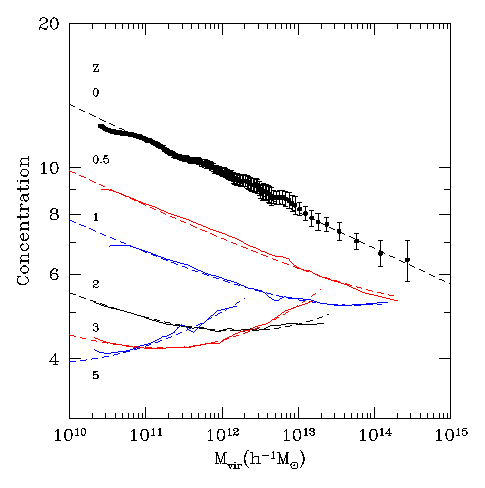
\includegraphics[width=\linewidth]{early_universe/klypin_2011_concentration_upturn.eps}
	\caption[Caption]{\footnotesize Caption.}
	\label{fig:concentration--klypin_concentration_upturn}
\end{figure}

\begin{figure}[ht]
	\centering
	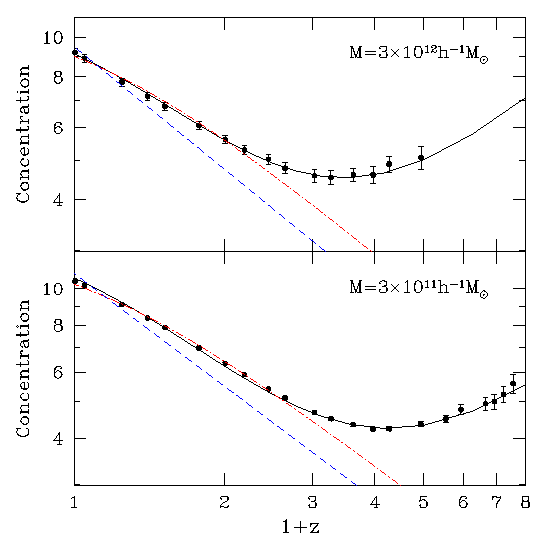
\includegraphics[width=\linewidth]{early_universe/klypin_2011_concentration_z_dependence.eps}
	\caption[Caption]{\footnotesize Caption.}
	\label{fig:concentration--klypin_concentration_z_dependence}
\end{figure}



%:::::::::::::::::::::::::::::::::::::::::::::::::::::::::::::::::::::::::::::::
\subsubsection{Substructure and Environment}
\label{subsubsec:early_universe--halo_properties--structure}
%:::::::::::::::::::::::::::::::::::::::::::::::::::::::::::::::::::::::::::::::


Text goes here.




%~~~~~~~~~~~~~~~~~~~~~~~~~~~~~~~~~~~~~~~~~~~~~~~~~~~~~~~~~~~~~~~~~~~~~~~~~~~~~~~
\subsection{Baryonic Processes}
\label{subsec:early_universe--baryonic_processes}
%~~~~~~~~~~~~~~~~~~~~~~~~~~~~~~~~~~~~~~~~~~~~~~~~~~~~~~~~~~~~~~~~~~~~~~~~~~~~~~~


Early-forming dark matter halos provide an incubator for the baryonic processes that transform the surrounding space and allow galaxies to form.  Initial gas accretion can lead to the formation of the first Pop-III stars \citep{1986MNRAS.221...53C, 1997ApJ...474....1T, 2000ApJ...540...39A, 2002Sci...295...93A}, which, upon their death, can collapse into the seeds for supermassive black holes (SMBHs) \citep{2001ApJ...551L..27M, 2003MNRAS.340..647I, 2009ApJ...701L.133A, 2012ApJ...754...34J} or enrich the surrounding medium with metals through supernovae \citep{2002ApJ...567..532H, 2003ApJ...591..288H}.  The radiation from these early quasars \citep{1987ApJ...321L.107S, 1999ApJ...514..648M, 2001AJ....122.2833F}, Pop-III stars \citep{1997ApJ...486..581G, 2003ApJ...584..621V, 2006ApJ...639..621A}, and proto-galaxy stellar populations \citep{2012ApJ...752L...5B, 2012MNRAS.423..862K} all play a key role in contributing to the re-ionizing the universe by around $z = 6$ \citep{2001PhR...349..125B}.  Additionally, halo mergers can drastically increase the temperature of halo gas through shock heating, increasing X-ray luminosity \citep{2009MNRAS.397..190S}, and contribute to the unbinding of gas to form the warm-hot intergalactic medium \citep{2008SSRv..134..141B, 2010MNRAS.405L..31S, 2012MNRAS.425.2974T}.



%:::::::::::::::::::::::::::::::::::::::::::::::::::::::::::::::::::::::::::::::
\subsubsection{The First Stars}
\label{subsubsec:early_universe--baryonic_processes--first_stars}
%:::::::::::::::::::::::::::::::::::::::::::::::::::::::::::::::::::::::::::::::


Text goes here.



%:::::::::::::::::::::::::::::::::::::::::::::::::::::::::::::::::::::::::::::::
\subsubsection{Supermassive Black Holes}
\label{subsubsec:early_universe--baryonic_processes--smbhs}
%:::::::::::::::::::::::::::::::::::::::::::::::::::::::::::::::::::::::::::::::


Text goes here.



%:::::::::::::::::::::::::::::::::::::::::::::::::::::::::::::::::::::::::::::::
\subsubsection{Enrichment and the The Intergalactic Medium}
\label{subsubsec:early_universe--baryonic_processes--igm}
%:::::::::::::::::::::::::::::::::::::::::::::::::::::::::::::::::::::::::::::::


Text goes here.



%:::::::::::::::::::::::::::::::::::::::::::::::::::::::::::::::::::::::::::::::
\subsubsection{Reionization}
\label{subsubsec:early_universe--baryonic_processes--reionization}
%:::::::::::::::::::::::::::::::::::::::::::::::::::::::::::::::::::::::::::::::


Text goes here.




